% \begin{itemize}
% 	\item Gráfico que sugirió Harari

% 	\item Corrección del clima
	
% 	\item Eventos entre 0.5 y 1
	
% 	\item Tabla con resultados \emph{con los resultados del dataset que estás usando para todos los bines usuales arriba de 1 EeV, no de eventos, amplitud , fase y probabilidad en siderea. }
% \end{itemize}

\section{Sugerencia de Harari}

Durante la presentación de lo que hiciste el semestre pasado, Harari sugirió hacer un histograma de los eventos con respecto a la energía. Durante la presentación afirmé que los eventos del main array iban perdiendo sensibilidad a los eventos de menor energía, y que por eso se empezó a utilizar a todos los disparos. En la Fig.\ref{fig:harari} es observa que también la sensibilidad disminuye a medida  que pasan los años en los eventos de todos los disparos. 

\begin{figure}[H]
	\centering
	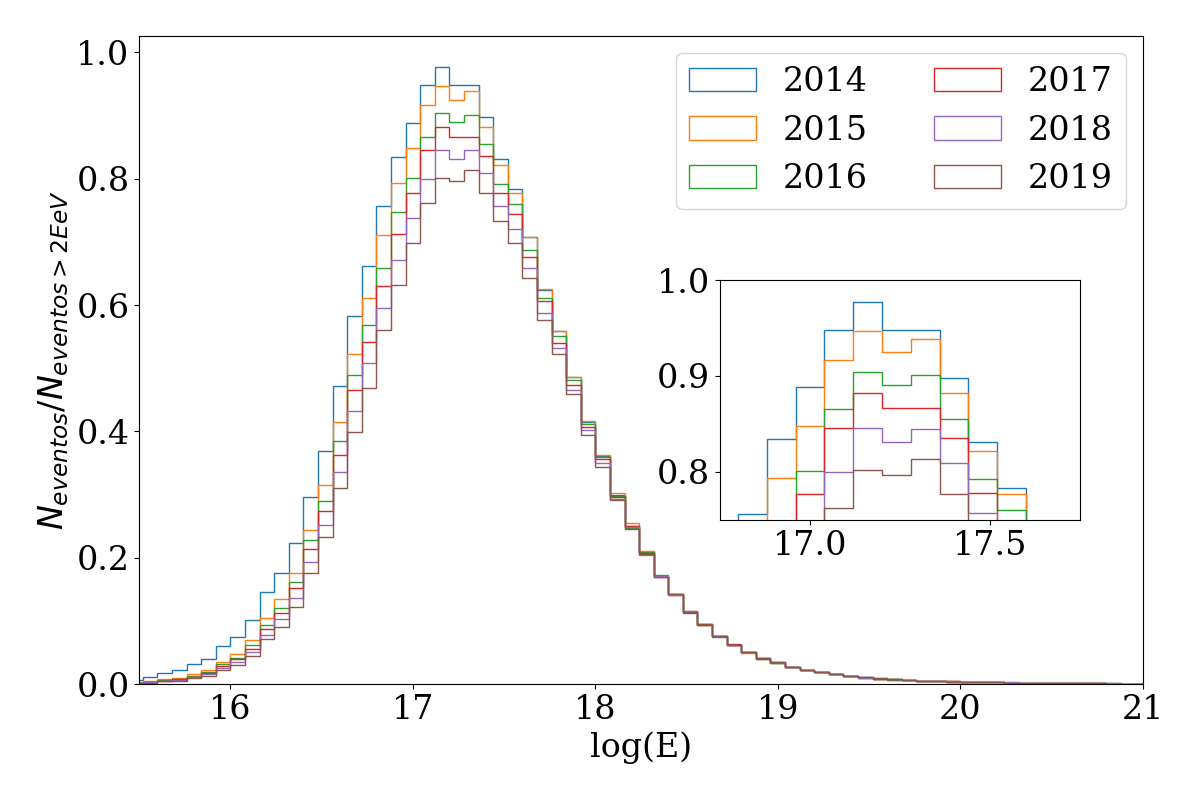
\includegraphics[width=0.5\textwidth]{figura_harari.png}
	\caption{La figura  sugerida por Harari}
	\label{fig:harari}
\end{figure}

En la siguiente tabla se muestra la cantidad de eventos y la energía media de cada año considerado:

\begin{table}[H]
\centering
\begin{tabular}{c||c|c}
Año & Eventos & ${log_{10}(E)}$ media [EeV]\\ \hline
2014& 2096481 & 17.12\\ \hline
2015& 1718141 & 17.17\\ \hline
2016& 1605716 & 17.18\\ \hline
2017& 1713876 & 17.20\\ \hline
2018& 1786301 & 17.24\\ \hline
2019& 1786301 & 17.28\\ \hline \hline
Total & 10706816 & 
\end{tabular}

\end{table}
\section{Parámetros del clima para los todos los disparos}

Para obtener los nuevos parámetros del clima, considero el conjunto de datos filtrado mediante el valor de $S_{38}=5.36\,$VEM sin la corrección de clima de la colaboración. Es es posible debido a que el archivo del Herald tiene los valores de $S(1000)$ sin corregir (columna 12) y los corregidos (columna 37), por lo tanto $S_{38}= S_{38,w}\nicefrac{S(1000)}{S(1000)_w} = \$12*\$47/\$37$. Este valor de $S_{38}$ de referencia corresponde aproximadamente a la energía de un evento 1 EeV. Considerando lo que había hecho durante la licenciatura, tenemos que:
\begin{align}
    S &= S_0 (1 + \alpha_P..+ \alpha_\rho*... + \beta_\rho...)\\
    \frac{dR}{d(sin^\theta)} &=  R_0 \big[ 1 + a_P.. + a_\rho ..+ b_\rho..  \big]
\end{align}
donde $S$ es la señal medida, $S_0$ la señal esperada, $\nicefrac{dR}{d(sin^\theta)}$ es la tasa de eventos por ángulo sólido, $R_0$ la tasa media y  $a_P = 2.363 \alpha_P$, también  los otros parámetros.


Para tener una idea si el modelo se ajusta a  lo observado experimentalmente, se consideran estos parámetros del clima independientes de $\theta$ y la tasa de eventos diaria, se obtiene el ajuste de la Fig.\ref{fig:tasa}. La media oscila alrededor  de $0.25$ eventos por $km^2$ por día, $\sim 56\%$ de aumento con respecto a la media de eventos para el \emph{disparo estándar}. 
\begin{figure}[H]
	\centering
	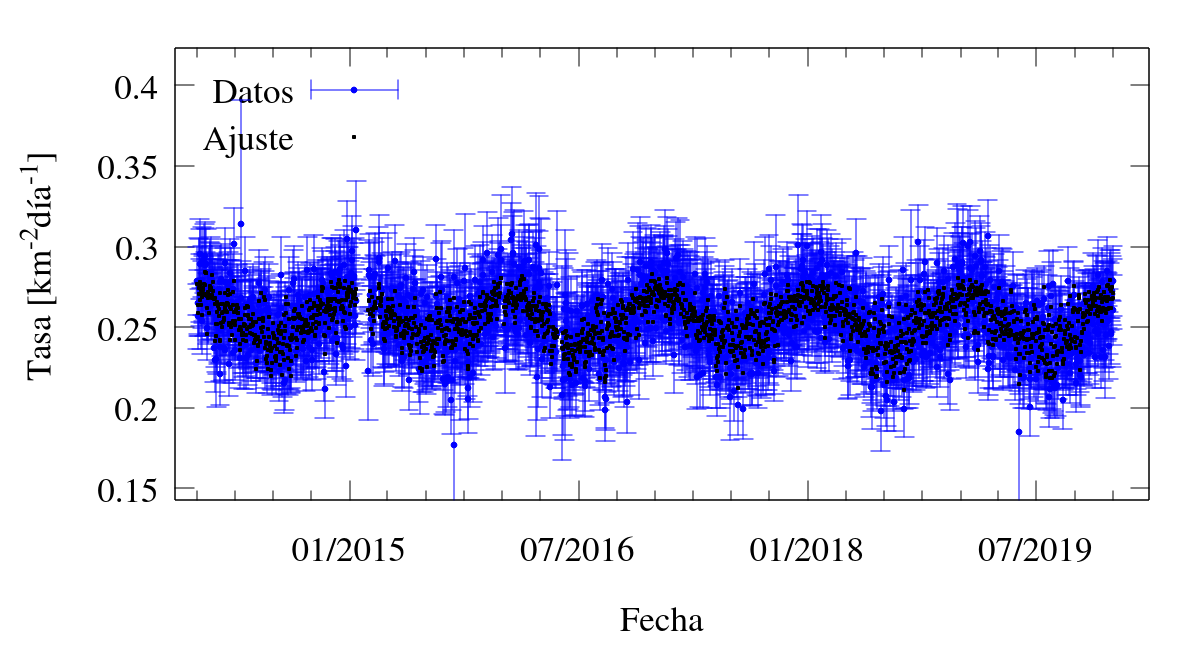
\includegraphics[width=0.5\textwidth]{figura_rate_durante_6_anhos.png}
	\caption{Tasa de eventos  por día por encima de $5.36\, \text{VEM} \sim 1 $\,EeV}
	\label{fig:tasa}
\end{figure}

Si hacemos un promedio de la tasa por cada hora durante los años 2014 al 2019, se obtiene la figura \ref{fig:hora}. Con respecto al disparo estándar se obtiene un curva de ajuste menos suave por la menor cantidad de años de eventos (por lo menos eso es lo que se me ocurre)
\begin{figure}[H]
	\centering
	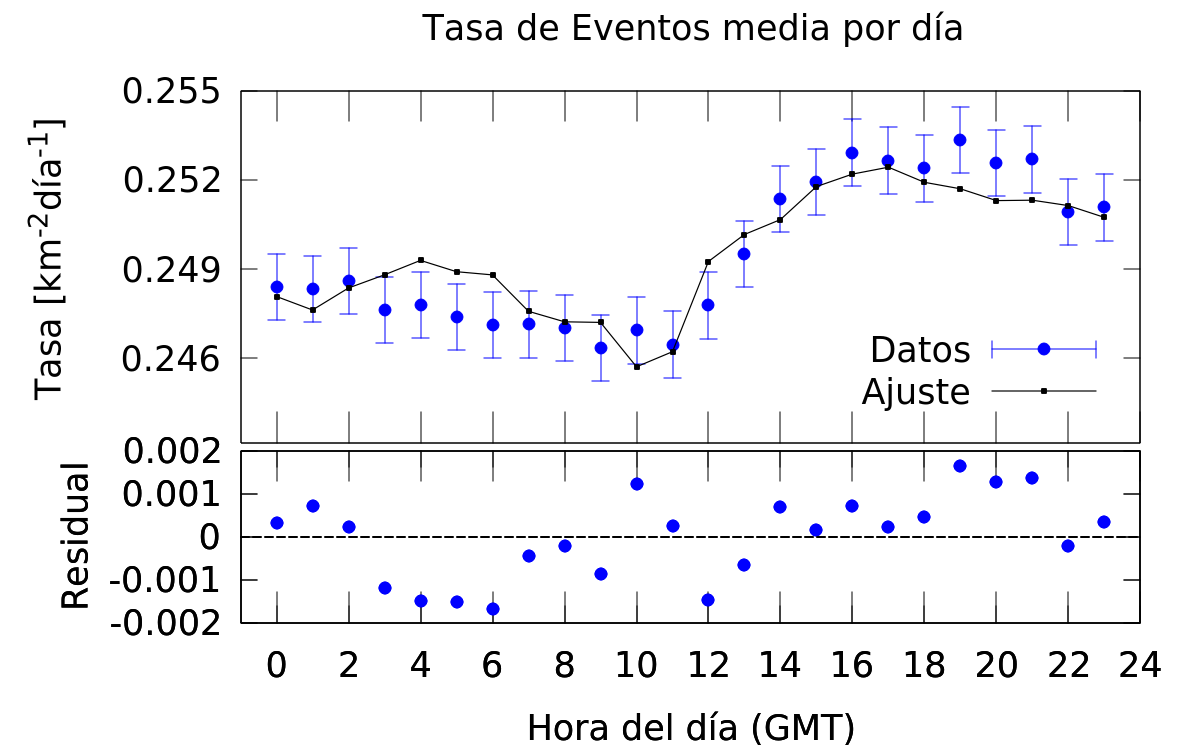
\includegraphics[width=0.45\textwidth]{figura_tasa_por_hora_del_dia.png}
	\caption{Tasa de eventos por hora por encima de  $5.36\, \text{VEM} \sim 1 $\,EeV}
	\label{fig:hora}
\end{figure}

Para los parámetros del clima en función del ángulo sólido, los ajustes obtenidos se presentan en las figs\ref{fig:ap}, \ref{fig:arho} y \ref{fig:brho}. Se comparan con los valores de la corrección del clima sobre el arreglo principal con el disparo estándar.


\begin{figure}[H]
	\centering
	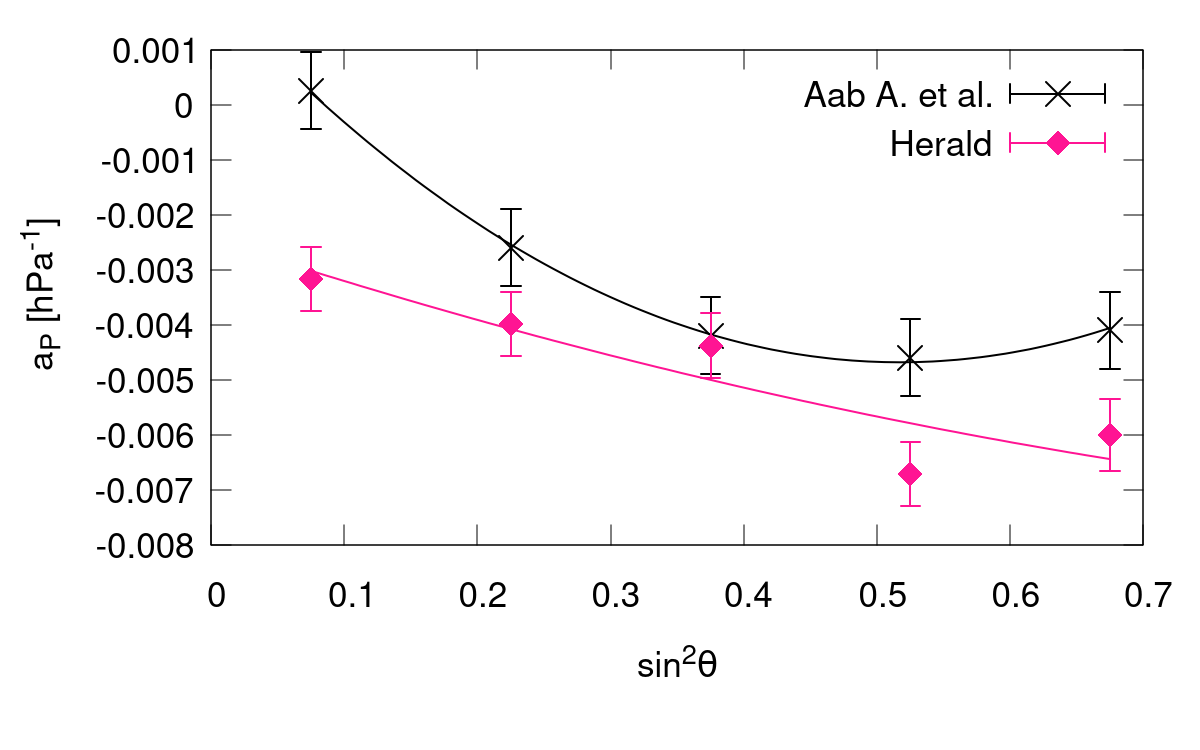
\includegraphics[width=0.5\textwidth]{figura_a_p.png}
	\caption{Parámetro de la presión}
	\label{fig:ap}
\end{figure}


\begin{figure}[H]
	\centering
	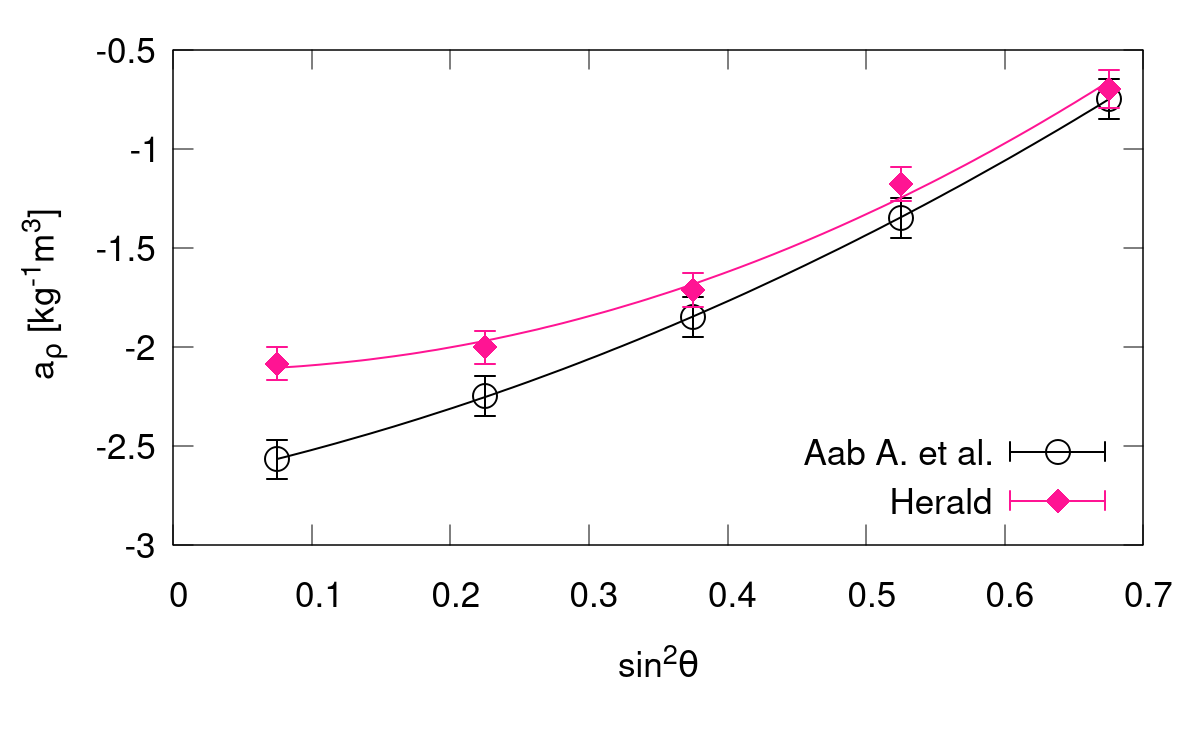
\includegraphics[width=0.5\textwidth]{figura_a_rho.png}
	\caption{Parámetro de la densidad del aire}
	\label{fig:arho}
\end{figure}

\begin{figure}[H]
	\centering
	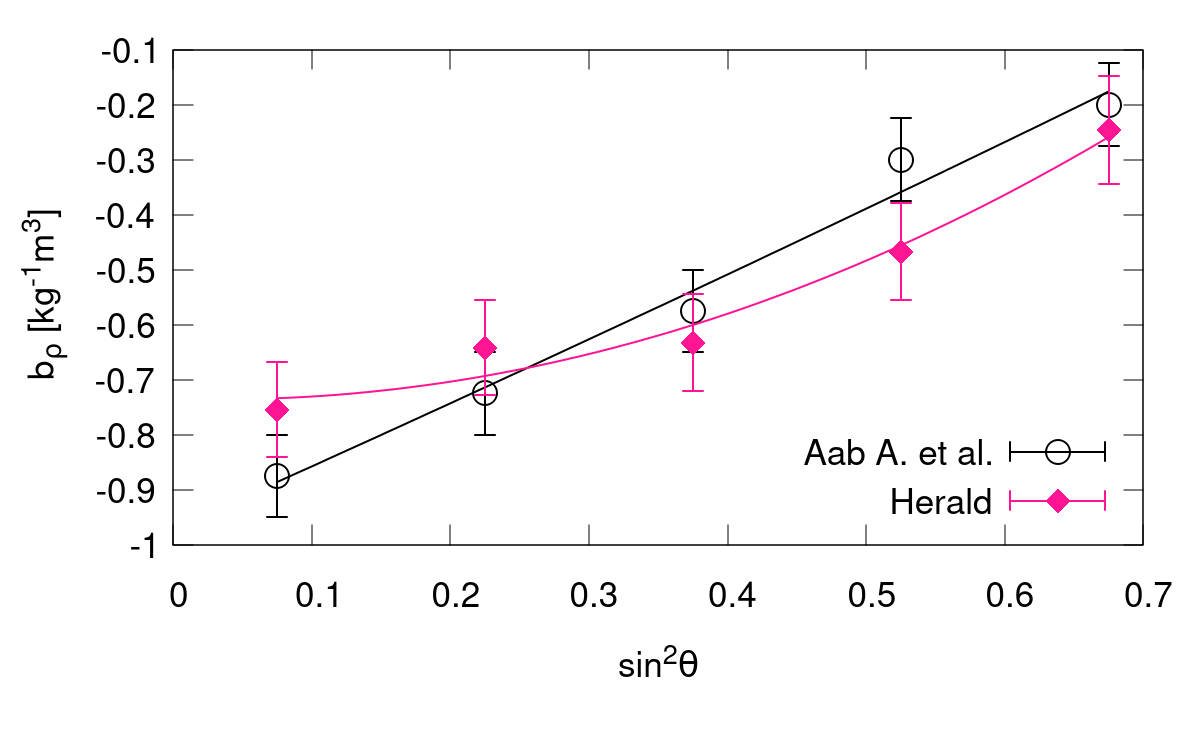
\includegraphics[width=0.5\textwidth]{figura_b_rho.png}
	\caption{Parámetro de la densidad del aire con el retraso de 2 horas}
	\label{fig:brho}
\end{figure}


\section{Corrección del clima}

Acá empezó a fallar todo y no sé que pasó, voy a detallar que errores (o cosas que me hace ruido) me salieron y que acciones tomé/ que detalles revisé para ver que sucedía.

En el informe de fin  de semestre, vimos que usando el bin  de 1 EeV - 2 EeV teníamos un Rayleigh sucio pero sin  la modulación diaria del clima (por lo menos no apreciable), como se muestra en la figura \ref{fig:sucio}



Esta figura solo tiene la corrección del clima con los parámetros de la colaboración obtenidos en el 2017, que además son utilizados por el disparo estándar.

Con los parámetros $a_P$, $b_\rho$ y $a_\rho$ en función de $\sin^2 \theta$ se hace un ajuste con un polinomio de orden 2. Por lo tanto, dado un evento, mediante el  valor de $\theta$ asociado podemos tener los parámetros del clima para corregir ese evento.



\begin{itemize}
\item Cuando preparo el archivo para la corrección, me aseguro de que se esté imprimiendo el valor de $S_{38}$ sin corregir.

\item Para obtener la señal $S_0$, que en este caso $S_{38,0}$, uso la expresión $S_{38,0} = S_{38}/(1 + \alpha_P..+ ...) = S_{38,w}\times \frac{S(1000)}{S(1000)_w (1 + \alpha_P..+ ...)  }$  

\item Con este valor $S_{38,0}$ reconstruyo la energía con $E=A (S)^B$

\end{itemize}



Como se ve en la Fig.\ref{fig:label}, la modulación diaria es muy grande con respecto a  lo que se vió el semestre pasado. Al momento de escribir esto, no encontré una razón por la cual sea tan grande el módulo. Lo que verifiqué son estos puntos

\begin{itemize}
	\item tomo el archivo que usé para calcular los parámetros
	\item Calculo la nueva energía
	\item Me restrinjo a los eventos entre 1 - 2 EeV según la energía nueva
	\item Hago el análisis en el mismo rango de tiempo que lo que presenté el semestre pasado.
\end{itemize}

\begin{figure}[htbp]
	\centering
	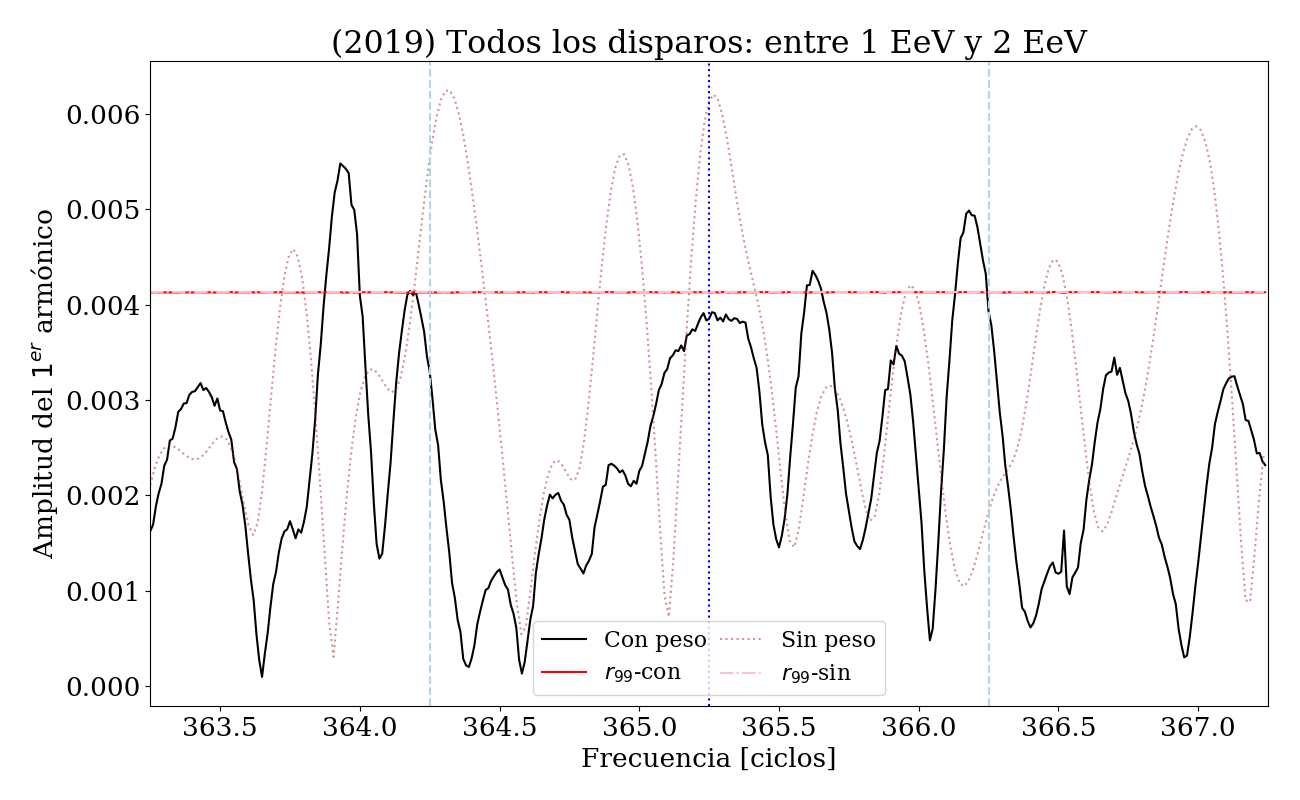
\includegraphics[width=0.5\textwidth]{/home/ponci/Desktop/TesisIB/Coronel/CodigoTesisIB/Update/6_Dipole_1-2_EeV/pesos_sin_con_1_2_EeV.png}
	\caption{Rayleigh con todos los disparos y la corrección de la colaboración}
	\label{fig:sucio}
--
\begin{figure}[H]
	\centering
	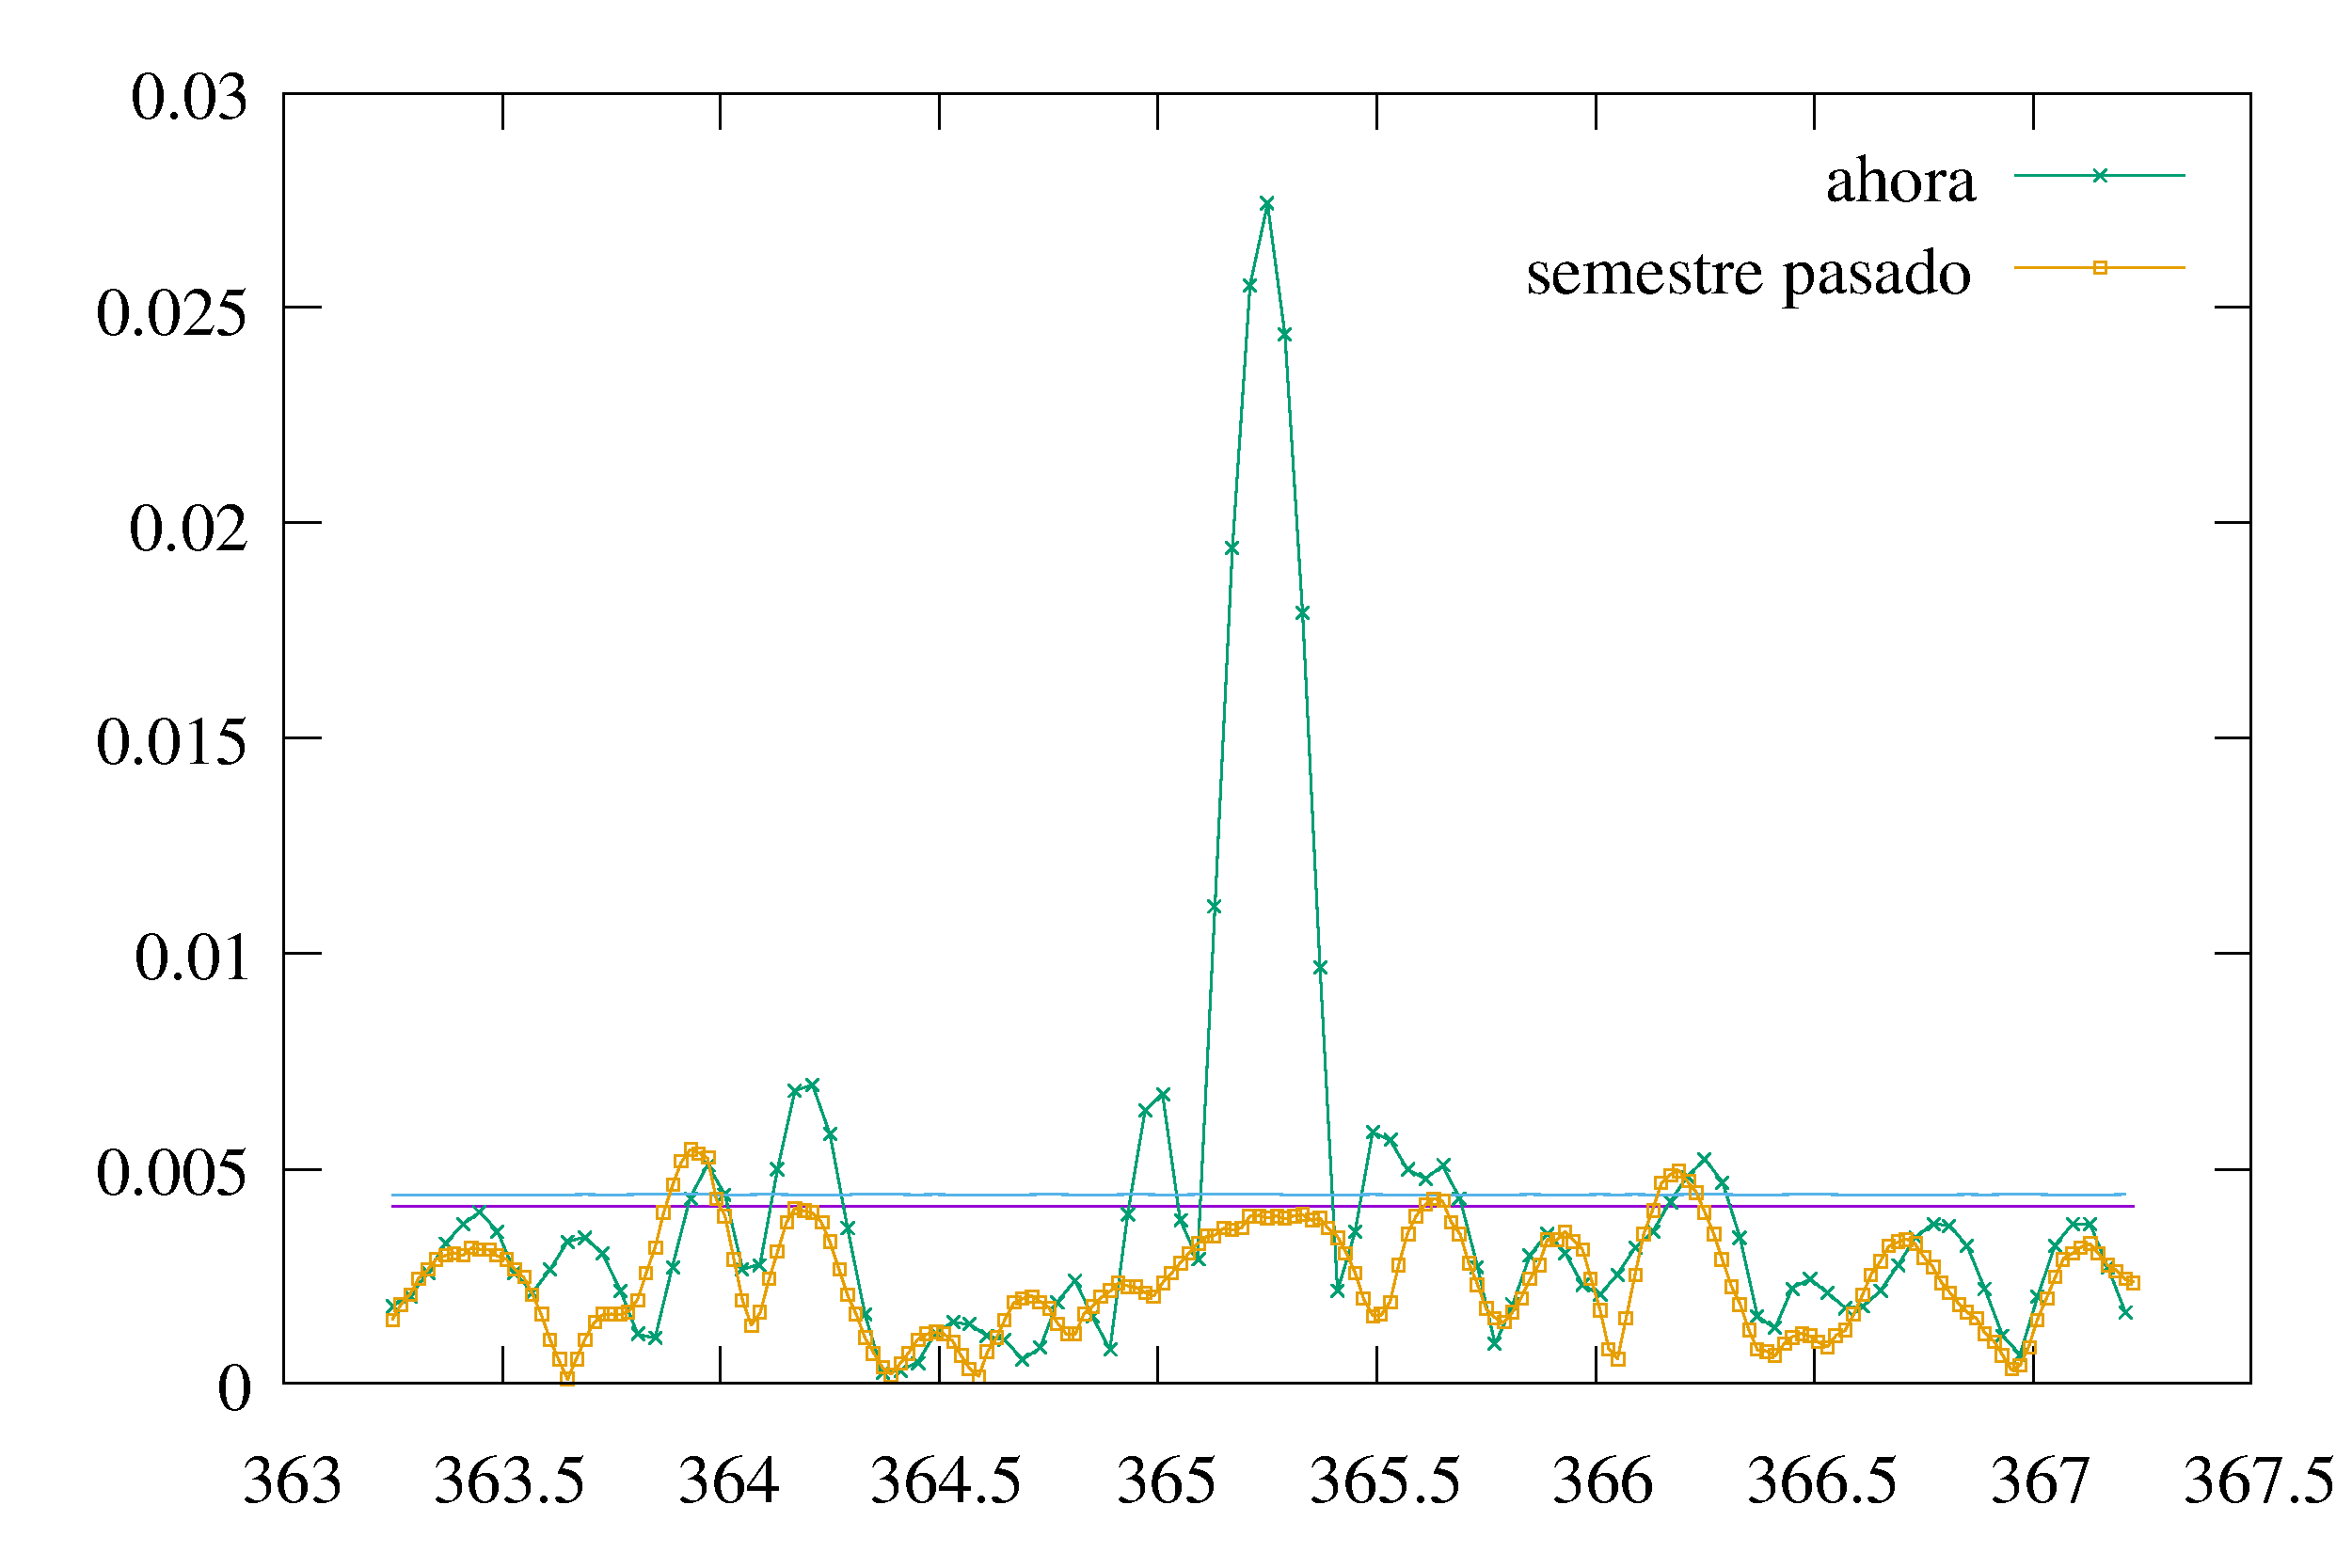
\includegraphics[width=0.5\textwidth]{sucio.pdf}
	\caption{ }
	\label{fig:label}
\end{figure}

\end{figure}